%Préambule
\documentclass[12pt]{report}

\usepackage[french]{babel}
\usepackage{luatextra}
\usepackage{hyperref}
\usepackage{hhline}
\usepackage{multirow}
\usepackage{listings}
\usepackage{caption}
\usepackage{amsmath}
\usepackage{enumitem} % listes à puces

\usepackage{lastpage}

\usepackage{fancyhdr}


\pagestyle{fancy}

\renewcommand{\thesection}{\Roman{section}}

%Information sur le document
\title{Projet d'Algorithmique \\ \textit{L'Ascenseur} }
\date{Mai-juin 2019}
\author{Victor \textsc{ALAIN} - Arthur \textsc{BLAISE} - Amélie \textsc{GUEDES} \\ - Loann \textsc{POTTIER}}

 \makeatletter
\let\theauthor\@author
\let\thetitle\@title
\let\thedate\@date
\makeatother

%En-tête
\fancyhead[L]{}
\fancyhead[C]{\rightmark}
\fancyhead[R]{}

%Pied-de-Page
\fancyfoot[L]{\thedate}
\fancyfoot[C]{\thepage\ / \pageref{LastPage}}
\fancyfoot[R]{\thetitle}

%Refonte du style des sections
\usepackage{titlesec}
\titleformat{\section}[display]
  {\normalfont\huge\bfseries\sffamily}
  {}
  {-15pt}
  {\LARGE}

\begin{document}

\renewcommand{\thesection}{\textbf{\arabic{section}}} % Supprimer les numéros de chapitres dans la table des matières

\maketitle
\tableofcontents

\clearpage


\section{Introduction}

\subsection{Avant-propos}
	Le jeu de l'ascenceur est un jeu de cartes complexe qui nécessite, pour y jouer, de bien maîtriser les règles. Pour reproduire ce jeu il nous fallait donc évidemment savoir y jouer, c'est dans ce but que nous avons essayé de synthétiser les règles essentielles à la création de l'algorithme. L'une des difficultés majeures a sans doute été la distribution des points à la fin de chaque manche, ou le listage des cartes qu'il est possible de jouer.\\
	
	Mais au final, cette partie réelle nous a permis de relever les points importants, et d'avoir une schématisation plus concrète du déroulement du jeu. Nous avons essayé de résumer les étapes principales du développêment ici.

	
\subsection{Problèmes à résoudre}
	
	Le but de ce projet est de réaliser un algorithme permettant d'exécuter le jeu de l'Ascenseur. Voici la liste des problématiques qui se sont présentées :\\
	
	\begin{itemize}[label=\textbullet, font=\LARGE]
		\item La première partie concerne la configuration du jeu : en effet il existe plusieurs variantes des règles, comme le nombre de joueurs, ou le nombre de points gagnés par manche... Il nous faut donc trouver un moyen pour laisser aux joueurs la possibilité de les modifier.
		
		Ce moyen a pris la forme d'un fichier config.txt qui résume sept options différentes : le nombre maximal de joueurs (humains et bots), le nombre de points gagnés par défaut à une manche remportée, le nombre de points gagnés ou perdu par pli, la taille en pixels de la fenêtre de jeu, et les limites d'âge des joueurs (qui sont demandées pour départager les joueurs).\\
		
		\item Ensuite vient le développement d'une partie : gérer le nombre de manches par phase (qui varie en fonction du nombre de joueurs), le nombre de tours par manche, la distribution ou la remise des cartes... à ce stade même la question de qui doit recevoir ses cartes en premier semble complexe.
		
		Lors d'une manche il faut aussi compter le nombre de plis remportés par chaque joueur, sans oublier de lui demander son pari au début. De surcroît chaque joueur ayant remporté une manche doit débuter la manche suivante. Il est important également de contrôler quelle carte chaque personne joue, pour vérifier que la couleur soit bien valide. Chaque joueur joue une carte de la couleur demandée s'il en possède une, sinon il doit jouer un atout. Cependant, un joueur n'est pas obligé de poser un atout s'il n'a pas de carte de la même couleur, il peut déposer une carte quelconque mais il perdra le tour. Il est aussi à noter que les jokers n'ont pas été inclus dans le jeu.\\
		
		\item La fin de la partie est heureusement simple à créer : le joueur ayant le plus de points gagne, point final.\\

		\item En annexe, une autre partie de code est ajoutée : la gestion des bots. Maintenant que les humains peuvent jouer, il faut leur permettre de jouer contre un ordinateur. C'est une partie assez ardue à modéliser puisqu'il faut prévoire plusieurs 'personnalités' d'Intelligence Artificielle, et créer l'algorithme correpondant.
	\end{itemize}
	
	\begin{figure}[h]
	\centering
	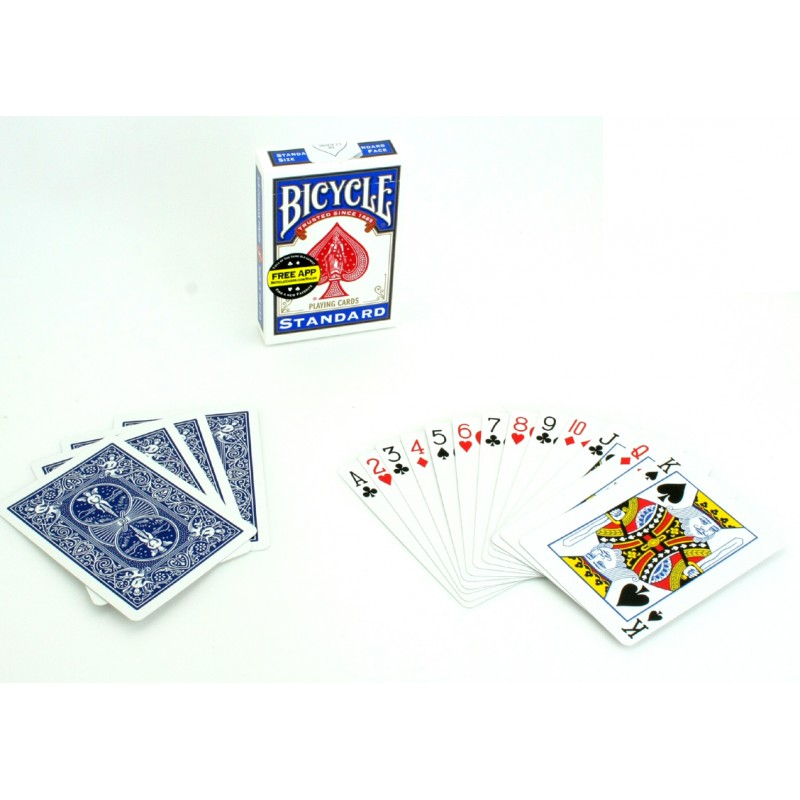
\includegraphics[scale=0.25]{jeu-de-cartes.jpg}
	 \caption{Jeu de carte utilisé lors d'une partie d'ascenseur}
	\end{figure}
		

		
\clearpage

		
\section{Explication des algorithmes}
Pour commencer, voici comment est construit le code. Tout part d'un programme principal \textit{start.pas} : c'est ce programme qui lance toutes les fonctions secondaires et les appellent dans le bon ordre, afin de permettre le bon déroulement du jeu. De surcroît ce programme utilise des unités, chacune s'occupant d'une partie spécifique du jeu.
  	\subsection{Structure du programme}
  
   \subsubsection{Programme principal}
   Le programme principal \textit{start.pas} demande à chaque joueur de renseigner son pseudo et son âge, qui seront utilisés dans le reste de la partie. Dans ce programme il y a également l'utilisation des \textit{unités}, ce qui évite d'avoir un fichier trop long (en segmentant le code, il devient plus lisible, et plus facile à tester). \\
   
   Ensuite, durant le déroulement du programme les choses se complexifient car le déroulement du jeu est définit dans deux unités. L'une demande si le joueur souhaite afficher les règles (unit \textit{intro.pas}), et l'autre contient chaque étapes du jeu (unit \textit{deroulement.pas}). \\
   
 Afin d'assurer le déroulement visuel du jeu l'aspect graphique est contenu dans une autre unité : \textit{graph.pas}. Celle-ci fonctionne un peu comme une lib graphique spécialement conçue pour le jeu de l'Ascenceur, en appelant d'elle même les unités gLib2D, SDL et autres. Le fait de l'avoir concentrée en un seul fichier permet de ne pas avoir trop d'appels ou d'imports dans le reste du code. Dans ce même but, l'unité \textit{classes.pas} rassemble toutes les classes utilisées dans le jeu.
 \clearpage
   
   \subsection{Unités utilisées}

   	\subsubsection{Introduction}
   	Cette unité est particulièrement simple car elle se contente de proposer à l'utilisateur la lecture des régles du jeu. Rapide et efficace.
   	
 	\subsubsection{Déroulement}
  Cette unité est initalement le coeur du programme; elle fait donc appel à 11 fonctions et 9 procédures différentes. Ces dernières sont : \\
  
  \begin{description}
  \item[Initjoueur:] Demande le nombre de joueurs présent dans la partie 
  \item[Initplimanche:] Permet de ramener le nombre de plis des joueurs a zéro avant la nouvelle manche
  \item[Inarray:] Vérifie la présence d'une carte dans la liste
  \item[Init:] Créé le paquet de carte 
  \item[Distribuer:] Distribue les cartes aux joueurs et empêche le doublon de carte
  \item[InitAtout:] Permet d'initialiser la couleur de la carte de l'atout
  \item[NombreManche:] Calcul le nombre de manches nécessaires vis-à-vis du nombre de joueur
  \item[VerifcouleurExiste:] Vérifie la couleur de cartes séléctionner par le joueur
  \item[VerifvaleurExiste:] Vérifie la valeur de la carte choisie
  \item[VerifieCareAjoueur:] Vérifie que le joueur possède la carte qu'il a selectionné 
  \item[ChoixCarte:] Applique les verifications sur le choix des cartes 
  \item[VerifDroitDePoser:] Vérifie si la cartes peut-être poser sans enfreindre les régles 
  \item[Pli:] A la fin d'un tour, renvoie un entier pour désigner le gagnant 
  \item[RetirePaquet:] Retire la carte du paquet une fois sélectionner 
  \item[OrdreJoueur:] Permet de determiné et d'appliquer l'ordre de jeu des joueurs pour le prochain pli
  \item[AfficheScore:] Permet d'afficher les scores de chacun à chaque fin de manche
  \item[Manche:] Applique les etats d'une manche a savoir le nombre de cartes au joueurs et l'enregistrement des paris 
  \item[Ascendant:] Donne une carte de plus a chaque joueur
  \item[Descandant:] Retire une carte a chaque joueur 
  \item[ComptageDePoint:] Compte le nombre de point associé aux joueurs 
  \item[Creerjoueur:] Affiche le pseudo et l'âge du joueur
  \item[Partie:] Procédure permettant de jouer une partie (Ascendant et Descendant)
  \end{description}
  \vspace{15pt}
  
  \subsubsection{Unité graphique}
	
	C'est le morceau de code qui permet de gérer toute l'interface graphique : de l'affichage du fond d'écran jusqu'au clic sur une carte, en passant par la saisie des paris ou les animations discrètes, tout est géré ici puis appelé dans le programme.  
  
  \begin{description}
  	\item[init:] Initialise la fenêtre avec une taille, et crée la référence de l'image de fond
  	\item[set\_deck:] Initialise la liste des cartes présentes dans le deck
  	\item[set\_cartes\_main:] Définit les cartes dans les mains du joueur
  	\item[set\_joueur:] Définit le joueur qui doit être affiché en focus (indicateur en haut à gauche de la fenêtre)
  	\item[set\_fps:] Initialise le nombre d'images par seconde
	\item[convert\_carte:] Complète les informations d'une carte pour la rendre utilisable par la lib graphique
	\item[load\_players:] Complète les informations d'un joueur pour le rendre utilisable par la lib graphique
	\item[convert\_text:] Convertit un texte en élément graphique
	\item[convert\_couleur] Convertit une couleur en bits (utilisé par le terminal) en une couleur graphique
	\item[afficher\_cartes]: Affiche la liste de cartes définie par \textit{set\_deck}
	\item[afficher\_joueurs:] Affiche la liste des joueurs autours de la "table"
	\item[afficher\_background:] Affiche l'image de fond
	\item[afficher\_texte:] Affiche un message
	\item[refresh:] Rafraîchit l'affichage de la fenêtre
	\item[focus\_joueur:] Affiche le pseudo du joueur focus en haut à gauche de l'écran
	\item[afficher\_atout:] Affiche la couleur de l'atout actuel
	\item[afficher\_manche:] Affiche la liste des cartes définies par \textit{set\_main}
	\item[afficher\_cadre:] Affiche un cadre autour de la carte survolée par la souris 
	\item[on\_click:] Retourne la carte où le joueur a cliqué
	\item[saisir\_txt:] Demande à l'utilisateur de saisir du texte
	\item[afficher\_score:] Affiche le score des joueurs dans une zone blanche, au milieu de la fenêtre
  \end{description}
  \vspace{15pt}
  
  /subsubsection{IA}
  	\item[CreerBot:] Permet de créer les bots avec son age et son pseudo
	\item[PartieBot:] Demande le nombre d'IA souhaité
	\item[ChoixCarteCouleurBot:] Affiche une carte d'une couleur de L'IA en fonction de la carte jouée précédemment
	\item[ChoixCarteBotPrems:] Affiche une carte aléatoire quand l'IA commence à jouer le pli
	
\section{Difficultés}
	\subsection{Coeur du programme}
	La principale difficulté rencontrée fût dans le choix des fonctions à réaliser mais surtout comment réaliser certaines fonctions. De plus, une autre difficulté était au moment de relié notre unit à l'interface graphique car les données entre les deux programmes étaient relativement différente. Nous avons également eu du mal à démarrer car les règles énoncés n'étaient pas très claires et nous avions tous compris des règles différentes, surtout au niveau du comptage des points.
	
	\subsection{Unité grahique}
	La principale difficulté rencontrée lorsque nous avons commencé la partie graphique est l'installation : malgré de nombreuses heures de tests, il nous a été impossible d'utiliser la lib SDL sur nos ordinateurs personnels. Cela nous a donc forcé à la travailler uniquement depuis les postes de l'école, ralentissant la progression de cette section du programme.\\ 
	
	D'autres problèmes sont apparus au fur et à mesure du code : par exemple il fallait pouvoir modifier la taille de la fenêtre afin de l'adapter à la taille de l'écran, ce que ne proposait pas nativement gLib2D. Nous avons donc dû modifier cette unité pour ajouter une fonction qui modifie l'échelle de la fenêtre, elle-même appelée par la procédure \textit{init}. \\
	\clearpage
	Certains défis se sont révélés intéressants à relever. Comment afficher les 52 cartes différentes sans avoir à les sauvegarder une par une sous forme d'image ? Nous avons opté pour la formation d'un rectangle blanc avec du texte superposé pour afficher la valeur et la couleur. Comment afficher les cartes, joueurs et autres items plus de 50 fois par seconde sans mettre à plat la mémoire libre de l'ordinateur ? Ils sont générés une seule fois puis stockés dans une variable de l'unité. Comment demander à l'utilisateur de saisir du texte ? Nous affichons une sous-fenêtre invitant l'utilisateur à écrire, puis on interrompt le programme afin de détecter les clics sur le clavier et afficher le résultat en temps réel. Et encore bien d'autres...

\vspace{15pt}
\section{Avantages et limites}


\section{Contribution des étudiants}
\subsection*{Arthur Blaise}
	Arthur s'est concentré sur l'utilisation de l'unité gLib2D, et la création de la lib graphique, pour pouvoir l'implémenter plus tard dans le programme. En annexe, il y a aussi eu la gestion du fichier de configuration.
	
\subsection*{Amélie Guedes et Victor Alain}
 Amélie et Victor se sont occupés du plus important, le coeur du programme. De la création des joueurs à la fin de la partie, en passant par le déroulé de chaque manche, chaque pli. 
 
\subsection*{Loann Pottier}
Loann a rejoint le projet en cours de route et, faute de pouvoir coder, s'est appliqué à comprendre le programme pour le résumer dans ce rapport.


\vspace{15pt}
\section{Bilan personnel}
\subsection{Amélie Guedes}

\subsection{Arthur Blaise}
Pour ma part, j'ai beau avoir une certaine expérience de la programmation, ce projet a été mon premier vrai travail avec une interface graphique. J'ai pu découvrir le monde du SQL, la gestion des événements, l'utilisation du cache pour limiter les fuites de mémoire, et plein d'autres choses passionnantes. Même si j'ai passé de longues heures à m'arracher les cheveux sur des problèmes d'apparence simples et à pester contre Pascal, je n'en reste pas moins fier du travail accompli. Ce jeu est tellement complexe à modéliser, sans même parler de l'affichage, que notre programme vallait la peine d'être créé. Et tant pis pour les longues heures noctures derrière mon ordinateur...

\subsection{Victor Alain}

De mon côté, ce projet m'a permis comme le précédent à m'améliorer en algorithmique, à penser différemment, à découvrir de nouvelles fonctionnalités. J'ai également appris comment départagé des algorithmes, c'est-à-dire à quel moment il faut faire plusieurs fonctions ... De plus, travailler en binôme à été bénéfique pour mieux comprendre les différents fonction ou procédures, mais également pour corriger les fautes que l'on pouvaient faire. Notre méthode de travail a également été différente et je ne fonctionnais pas comme cela auparavant. En effet, nous avons commencé par la procédure de fin et nous avons finis par la première fonction.

\subsection{Pottier Loann}

\section{Conclusion}

QUI AIME LES COOKIES ??? Bah tout le monde. 
			
\end{document}
